%TO RUN THIS FILE: setwd("C:\\Documents and Settings\\mark.vdwiel\\Desktop\\ShrinkBayes\\inst\\doc"); Sweave("ShrinkBayes.Rnw")

%\VignetteIndexEntry{ShrinkBayes}
%\VignetteDepends{}
%\VignetteKeywords{Bayesian analysis of high-dimensional omics data, either Gaussian or counts }
%\VignettePackage{ShrinkBayes}

\documentclass[11pt]{article}

\usepackage{amsmath}
\usepackage[authoryear,round]{natbib}
\usepackage{hyperref}


\newcommand{\para}{\bigskip\noindent}




\usepackage{Sweave}
\begin{document}

\setkeys{Gin}{width=0.99\textwidth}

\title{\bf ShrinkBayes: Bayesian analysis of high-dimensional omics data}

\author{Mark A. van de Wiel}

\maketitle

\begin{center}
Department of Epidemiology \& Biostatistics\\
VU University Medical Center\\
Amsterdam, The Netherlands
\end{center}

\begin{center}

{\tt mark.vdwiel@vumc.nl}
\end{center}


\tableofcontents

%%%%%%%%%%%%%%%%%%%%%%%%%%%%%%%%%%%%%%%%%%%%%%%%%%%%%%%%%%%%%%%%%%%%%%%%%%%
\section{Overview}
%NOTE: THIS VIGNETTE WILL BE UPDATED TO INCLUDE AN EXAMPLES ON TESTING NESTED MODELS THAT DIFFER BY MORE THAN ONE VARIABLE.

\para
ShrinkBayes is a package for Bayesian
(differential) expression analysis of high-dimensional -omics
data. It applies Emprical Bayes-type \emph{multi}-parameter
shrinkage to improve parameter estimation and inference.
You should use it because it

\begin{itemize}
\item Is very flexible in terms of study designs
\item Allows for random effects in a GLM setting
\item Applies to many different data types, including
Gaussian (e.g. miRNA, mRNA arrays, HT RNAi), counts (e.g.
label-free proteomics) and zero-inflated counts (e.g. AGE,
RNAseq)
\item Was demonstrated to be more reproducible and powerful than other methods in small-sample settings
    \citep{WielShrinkSeq,WielHTRNAi}
\item Is much more computationally efficient than MCMC, because it makes use of
INLA ({\tt www.r-inla.org}; \cite[]{Rue2009})
\item Provides (Bayesian) False Discovery Rates.
\end{itemize}

This document provides an overview on the usage of the ShrinkBayes package.
For more detailed information on the methodology, performance and assumptions we refer to the articles
\citep{WielShrinkSeq,WielHTRNAi,WielShrinkBayes}.
As example data we attached four data sets: 1) Simulated Gaussian data with 1500 rows and 284 columns; 2) HTRNAi, a data set with 960 rows and 6 columns containing Gaussian normalized HT RNAi
data; 3); and mirseqnorm, a data set containing miRNA sequencing-based counts with 2,060 rows (features) and 55 columns (samples); and
4) CAGEdata1000, with 10,000 rows (features) and 25 columns (samples) containing normalized sequencing-based counts.

\para
The simulated data set is used to illustrate the following aspects of ShrinkBayes:
\begin{itemize}
\item Ease of use in plain 2-group setting
\item Proof of concept: ShrinkBayes correctly identifies the prior effect size distribution
\item How to use a parametric mixture prior with point mass at zero?
\end{itemize}

\para
The HT RNAi data  set is used to illustrate the following aspects of ShrinkBayes:
\begin{itemize}
\item Analysis of Gaussian data (hence this example also covers most microarray data)
\item Use of an offset in your model
\item How to shrink multiple fixed effects and error variance?
\item Use of a non-symmetric prior
\end{itemize}

\para
The CAGE data set is used to illustrate the following aspects of ShrinkBayes:
\begin{itemize}
\item Analysis of (zero-inflated) count data (example also covers other sequencing data like RNAseq)
\item Dealing with a complex design, including nuisance factors and blocked individuals
\item Modeling and analysing random effects
\item Estimation and inference for multiple pair-wise comparisons
\item Joint shrinkage of fixed effect, random effect and overdispersion
\item Using a mixture distribution on overdispersion
\end{itemize}

\para
The miRNA sequencing data set was added to illustrate simple, one-line use of ShrinkBayes. In addition,
it illustrates $K$-sample testing for a factor with more than 2 levels.

\para
All examples use a fairly similar same work flow:
\begin{enumerate}
\item Load the normalized data
\item Set up the model and study design, possibly including multiple comparisons
\item Apply joint iterative procedure to shrink multiple parameters
\item Fit models for all data rows using the shrunken priors
\item Combine posteriors when multiple models have been applied to the same data (e.g. Poisson and Negative Binomial)
\item Update priors for crucial parameters to non-parametric or mixture forms
\item Update posteriors accordingly using the fitted non-parametric or mixture priors
\item Compute summaries like posterior means (parameter estimates) or posterior tail probabilities (local false discovery rates)
\item Compute Bayesian False Discovery Rates
\end{enumerate}

For the analysis of the HTRNAi and CAGE data sets we focus on illustrating the settings as used in \citep[HT RNAi data]{WielHTRNAi} and
\citep[CAGE data]{WielShrinkSeq}, but will also discuss alternatives when appropriate.

\section{Pre-amble: Accounting for different library sizes}\label{offset}
ShrinkBayes does NOT automatically account for different library sizes. There are two solutions. 

\begin{enumerate}
\item Create normalized (pseudo-)counts from the $p \times n$ counts matrix and apply ShrinkBayes to those:
\begin{Sinput}
> libsize <- colSums(counts)

#library size relative to geometric mean
> rellibsize <- libsize/exp(mean(log(libsize))) 

> pseudocounts <- round(sweep(counts, 2, rellibsize, "/"))
\end{Sinput}
\item Use the original counts, but include sample specific offsets that relate to the library sizes in the model (e.g. a simple model with an intercept and a
group variable, see further on for other examples):
\begin{Sinput}
> libsize <- colSums(counts)
> rellibsize <- libsize/exp(mean(log(libsize))) 
> myoffsets <- log(rellibsize)
> form <- ~ 1 + group + offset(myoffsets)
\end{Sinput}
\end{enumerate}
We prefer the second solution, although the first may sometimes be convenient when the data is also used for other purposes than testing (e.g. classification or prediction),
which would also require normalized data. 


\section{Example 0, Easy Start: ShrinkBayes in one line}
Please try the following example.

\para
\begin{Schunk}
\begin{Sinput}
> library(ShrinkBayes)
> data(mirseqnorm)
> head(mirseqnorm[,1:10])
\end{Sinput}
\begin{Soutput}
  M1 M10 M11 M12_1 M12_2 M13 M14_1 M14_2 M15 M16
1  0   0   0     0     0   3     0     0   2   0
2  0   0   0     0     0   0     0     0   0   0
3  0   0   0     0     0   0     0     0   0   0
4  0   0   0     0     0   0     0     0   0   0
5  1   0   0     0     0   0     0     3   1   0
6  0   0   0     0     0   0     0     0   0   0
\end{Soutput}
\end{Schunk}
Loads the package and the data.

\para
\begin{Schunk}
\begin{Sinput}
> data(designmirseq)
> head(designmirseq)
\end{Sinput}
\begin{Soutput}
  PM indiv timepos chemo organ1 organ2 organ3  organ
1  M     1       1     1      0      1      0 organ2
2  M    10       0     0      0      0      1 organ3
3  M    11       0     0      0      0      0 organ0
4  M    12       1     0      0      0      0 organ0
5  M    12       1     0      0      1      0 organ2
6  M    13       1     0      0      1      0 organ2
\end{Soutput}
\end{Schunk}
Show the design of the study.

\para
\begin{Schunk}
\begin{Sinput}
> PM <- designmirseq$PM
> indiv <- designmirseq$indiv
> timepos <- designmirseq$timepos
> chemo <- designmirseq$chemo
> organ <- designmirseq$organ
\end{Sinput}
\end{Schunk}
Retrieve relevant covariates

\para
\begin{Schunk}
\begin{Sinput}
> form = ~ 1 + PM + timepos + chemo + organ + f(indiv)
\end{Sinput}
\end{Schunk}
Specifies the regression formula. Note that f() is used to define a random effect. Please consider
including offsets (see Section \ref{offset}) when your data has different library sizes!
Then, a one-line application of ShrinkBayes is (but try the one below for a quick test):
\para
\begin{Schunk}
\begin{Sinput}
> SBmir <- ShrinkBayesWrap(mirseqnorm,form)
\end{Sinput}
\end{Schunk}
This performs shrinkage and testing for the FIRST variable in \texttt{form}, \texttt{PM}. If testing is desired for a different
variable this may be specified in the \texttt{paramtotest} argument (see below). The result is a list object with for slots.
The FDRs slot contains the FDRs for the \texttt{PM} factor, the local fdrs and the shrunken effect size estimate (P-M). The nsigsFDR01 slot
contains the number of significant results at (B)FDR threshold 0.1. The other two slots contain information on the
(shrunken) priors.

\para
For a relatively quick try, try the following:
\begin{Schunk}
\begin{Sinput}
> SBmirsmall <- ShrinkBayesWrap(mirseqnorm[1:100,],form,
+ ntag=c(25,50),maxiter=2,priorsimple=TRUE, approx0=TRUE)
\end{Sinput}
\end{Schunk}
Here, using a smaller data set, less iterations, a simpler prior (pointmass-Gauss) and an approximation of the null-model speeds up the computations.


\para
If you wish to shrink additional parameters as well (can render more powerful testing, in particular when sample size is small \citep{WielHTRNAi}), you may do so
by specifying these:
\begin{Schunk}
\begin{Sinput}
> SBmirshrink <- ShrinkBayesWrap(mirseqnorm,form,
+ shrinkaddfixed=c("organ","chemo","timepos"))
\end{Sinput}
\end{Schunk}

\para
A (marginal)-likelihood-ratio-based test for \texttt{organ} (which has four levels) is the default for factor variables with more
than 2 levels:
\begin{Schunk}
\begin{Sinput}
> SBmirorgan <- ShrinkBayesWrap(mirseqnorm,form,paramtotest="organ")
\end{Sinput}
\end{Schunk}


\para
What does \texttt{ShrinkBayesWrap()} do? It is just a wrapper for functions that are explained in more detail in the remainder of this document.
These functions are \texttt{ShrinkSeq()} and \texttt{ShrinkGauss()} for simultaneous shrinkage (Count and Gaussian data, respectively); \texttt{FitShrinkAll()} for applying \texttt{INLA}
to all data rows;  \texttt{MixtureUpdatePrior()}, \texttt{MixtureUpdatePosterior()}  and \texttt{BFUpdatePosterior()} for computation
of a prior with point mass and posteriors; \texttt{SummaryTable()} for computing summaries (including FDRs) from the posteriors.

\para
For a factor variable with more than 2 levels, it performs (marginal)-likelihood-ratio-based $K$-sample testing by default, but multiple comparisons
can be performed by use of either of the arguments \texttt{allcontrasts} or \texttt{multvscontrol}. See also \texttt{?ShrinkBayesWrap} for another example.


\section{Example 1: Gaussian simulation setting, 2-group setting}\label{simul}
\subsection{Workflow}
The example data set contains 1500 rows (features) and 8 samples (divided in two groups of 4).
The first 1000 represent non-differential features (so proportion non-differential equals 2/3), the
last 500 represent differential features with mean group difference simulated from a $N(0,1)$ distribution.
The noise is simulated from a $N(0,0.5^2)$ distribution.
See Section \ref{simulation} for the code used to simulate the data.

\para
\begin{Schunk}
\begin{Sinput}
> library(ShrinkBayes)
> data(datsim)
> head(datsim[,1:5])
\end{Sinput}
\begin{Soutput}
            [,1]         [,2]       [,3]        [,4]       [,5]
[1,] -0.04191917  0.070037754  0.8198383 -0.35443640  0.1128436
[2,] -1.01134453 -0.235494343 -0.3670104 -0.53177746  0.3673819
[3,]  0.19333209 -0.008211341 -0.1544538  0.29010757 -0.1937141
[4,] -1.03722998 -0.391160705 -0.2452836 -0.98763216 -0.8069727
[5,] -0.40153756  0.040684804  0.5219447 -0.09762872  0.1809304
[6,] -0.82760690  0.706451170  1.0892873  0.55709375  0.3335727
\end{Soutput}
\end{Schunk}
Loads the package and the data.

\para
\begin{Schunk}
\begin{Sinput}
> ncpus2use <- 10
\end{Sinput}
\end{Schunk}
Sets the number of cpus to use for parallel computations. Combined
with the {\tt ncpus=ncpus2use} argument in the functions this fixes the number of cpus used.
Note that for all functions the default is 2. If ncpus2use is larger than the actual
number of available cpus, computations will still run.

\para
\begin{Schunk}
\begin{Sinput}
> group <- factor(c(rep("group1",4),c(rep("group2",4))))
\end{Sinput}
\end{Schunk}
Defines covariate ``group'', corresponding to the columns of the datsim data.

\para
\begin{Schunk}
\begin{Sinput}
> form = y ~  1 + group
\end{Sinput}
\end{Schunk}
Define the model formula. Specification should be according to the {\tt inla formula} argument.


\para
\begin{Schunk}
\begin{Sinput}
> shrinksimul <- ShrinkGauss(form=form, dat=datsim,shrinkfixed="group",
+ ncpus=ncpus2use)
\end{Sinput}
\end{Schunk}

This function simultaneously shrinks the fixed effect parameter
`group' and the Gaussian error standard deviation (default), using standard
parametric priors.
The function may take considerable computing time. See Section
\ref{htrnai} for discussion on a) some arguments of the
ShrinkGauss function b) retrieving various types of information
from {\tt shrinksimul}.


\para
\begin{Schunk}
\begin{Sinput}
> fitg <- FitAllShrink(form,dat=datsim,fams="gaussian",shrinksimul,
+ ncpus=ncpus2use)
\end{Sinput}
\end{Schunk}
Applies {\tt inla} to compute posteriors for all data rows using the priors stored in {\tt shrinksimul}. IMPORTANT:
for better performance in the next function ({\tt MixtureUpdatePrior}), the prior for the {\tt shrinkfixed} parameter as
used in {\tt ShrinkGauss} (here: ``treatment'') is by default dispersed by a factor 10 (hence a vaguer prior is used),
see Section \ref{htrnai}.

\begin{Schunk}
\begin{Sinput}
> form0 = y ~  1
\end{Sinput}
\end{Schunk}
Defines the null-model formula. Specification should be according to the {\tt inla formula} argument.


\begin{Schunk}
\begin{Sinput}
> fitg0 <- FitAllShrink(form0,dat=datsim,fams="gaussian",shrinksimul,
+ ncpus=ncpus2use)
\end{Sinput}
\end{Schunk}
Fits the null-model. Only needed when inference for a point
null hypothesis is desired. Please note that, in principle, the
several UpdatePrior functions also work without a null-fit;
Then, the Savage-Dickey approximation is used to approximate
the marginal likelihood under the null- model. This saves
computing time, but can be less accurate.

Below we estimate a mixture
prior, namely a mixture of a zero point mass and two
non-central Normals: $\pi(\beta) =  (1-p_0)*p_{\text{min}} * N(\beta;
-\mu,\tau^2) + p_0 \delta_0 + (1-p_0)*(1-p_{\text{min}} ) * N(\beta; \mu,\tau^2)$. Note that this prior
is misspecified w.r.t. to true effect size distribution (pointmass + central Normal).

\begin{Schunk}
\begin{Sinput}
> mixtprior2gauss <-
+ MixtureUpdatePrior(fitall=fitg,fitall0=fitg0, modus="mixt",
+ shrinkpara="group",ncpus=ncpus2use)
\end{Sinput}
\end{Schunk}

\begin{Schunk}
\begin{Sinput}
> bestfinal <- mixtprior2gauss$allpara[1,]
> bestfinal
\end{Sinput}
\begin{Soutput}
        pmin           p0           mu        stdev    sumloglik
   0.3666667    0.6333333    0.1197843    0.9280651 1011.0476812
\end{Soutput}
\end{Schunk}

\begin{Schunk}
\begin{Sinput}
> mixtpostshr <- MixtureUpdatePosterior(fitg,mixtprior2gauss,fitg0,
+ ncpus=ncpus2use)
\end{Sinput}
\end{Schunk}
Update the posteriors of the {\tt "group"} parameter for all data rows using the mixture prior.

\begin{Schunk}
\begin{Sinput}
> lfdrless <- SummaryWrap(mixtpostshr, thr = 0, direction="lesser")
> lfdrgreat <- SummaryWrap(mixtpostshr, thr = 0, direction="greater")
\end{Sinput}
\end{Schunk}
Compute posterior (tail-)probabilities under shrinkage prior.
Here {\tt lfdrless =} $P(\beta_{\text{group}} \leq  0 | Y)$ and {\tt lfdrgreat =} $P(\beta_{\text{group}} \geq  0 |Y)$ are computed.
These can be interpreted as local false discovery rates corresponding to a one-sided interval null-hypothesis
$H_0: \beta_{\text{group}} \leq  0$ (for {\tt lfdrless}) or $H_0: \beta_{\text{group}} \geq  0$ (for {\tt lfdrgreat}). See
\citep{WielShrinkSeq}. Practically: if for a given feature {\tt min(lfdrless,lfdrgreat)} is small, it means that the posterior
is largely concentrated on either side of zero, wich indicates that the group effect is different from 0. This fact is used
when computing our {\it two-sided} version of Bayesian False Dicovery Rate \citep[BFDR]{Ventrucci, WielShrinkSeq}:


\begin{Schunk}
\begin{Sinput}
> BFDRs <- BFDR(lfdrless,lfdrgreat)
\end{Sinput}
\end{Schunk}
Computes two-sided BFDRs. These can be interpreted as false discovery rates (in a cumulative sense) when one would select all
features with smaller or equal null-probabilities (lfdrs) than the given feature.

\begin{Schunk}
\begin{Sinput}
> plot(BFDRs)
\end{Sinput}
\end{Schunk}
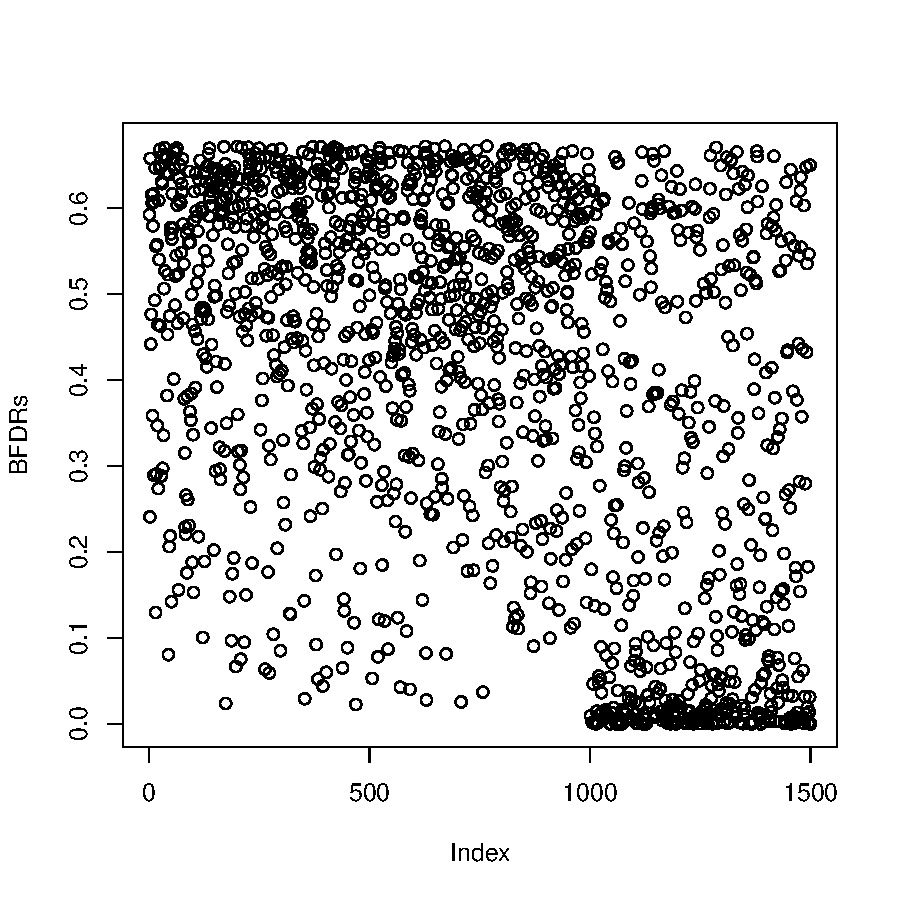
\includegraphics{ShrinkBayes-023}

\noindent
Plots the BFDRs against the feature index. Here we know that the first 1000 are generated from
the null-hypotheses, the latter 500 from the alternative (see Section \ref{simulation}).



\para
The computations above use a misspecified prior for $\beta_{\text{group}}$ (because it is actually simulated from
(\ref{gaussdirac}), the assumed model). Although it is fairly common to assume a fixed specific model in statistical computations,
it is worthwhile to explore alternatives. {\tt ShrinkBayes} offers two: 1) use a variety of parametric mixture models and study the robustness of the results
against the parametric shape of the prior; 2) use a nonparametric prior.
1) is explored in the next Section, 2) in Sections \ref{htrnai} and \ref{cage}.


In a simulation setting we can check the accuracy of the BFDR estimation to estimate the true FDR with the function {\tt fdrcomp}
(see Section \ref{truefdr}):

\begin{Schunk}
\begin{Sinput}
> res <- fdrcomp(1:1000,BFDRs)
> plot(res,type="l")
> abline(a=0,b=1,col="red")
\end{Sinput}
\end{Schunk}
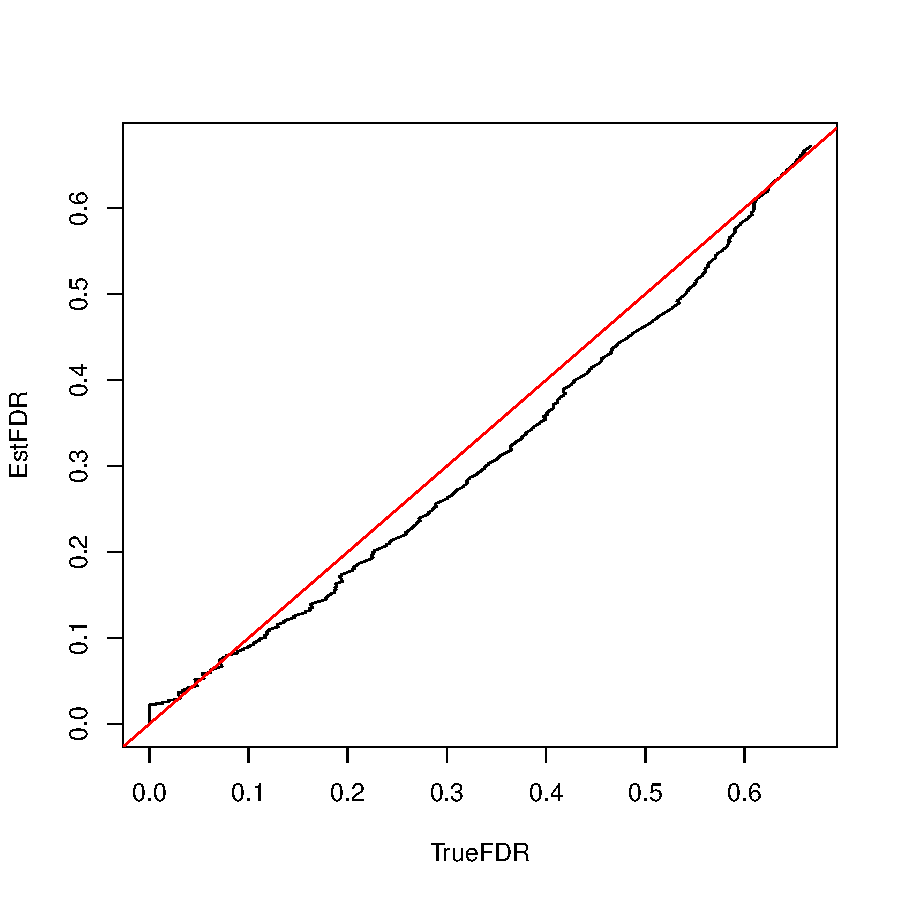
\includegraphics{ShrinkBayes-025}

\subsection{Results when using the correct prior}\label{correct}

%
\begin{Schunk}
\begin{Sinput}
> prior1Normalp0 <- MixtureUpdatePrior(fitall=fitg,fitall=fitg0,
+ modus="gauss", shrinkpara="group",ncpus=ncpus2use)
\end{Sinput}
\end{Schunk}
Finds the (approximately) best mixture prior of the form
\begin{equation}\label{gaussdirac}
\pi(\beta) = p_0 \delta_0 + (1-p_0) N(\beta; 0,\tau^2),
\end{equation} so a mixture of
zero-point mass (group effect equals zero) and a central Normal distribution. Grid search is used to maximize total
log marginal likelihood. Inclusion of a point mass may be attractive for the purpose of statistical inference
\citep{WielShrinkSeq}.

\begin{Schunk}
\begin{Sinput}
> bestfinal <- prior1Normalp0$allpara[1,]
> bestfinal
\end{Sinput}
\begin{Soutput}
          p0        stdev    sumloglik
   0.6000000    0.8460445 1010.0916223
\end{Soutput}
\end{Schunk}
The best values of the parameters. Note the good performance of the algorithm:
the true values are {\tt p0 = 0.67} and {\tt stdev = 1}.
Let us now recompute the posteriors, lfdrs and BFDRs
of $\beta_{\text{group}}$ under this prior:

\begin{Schunk}
\begin{Sinput}
> post1Normalp0shr <- MixtureUpdatePosterior(fitg,prior1Normalp0,fitg0,
+ ncpus=ncpus2use)
> lfdrless2 <- SummaryWrap(post1Normalp0shr, thr = 0, direction="lesser")
> lfdrgreat2 <- SummaryWrap(post1Normalp0shr, thr = 0, direction="greater")
> BFDRs2 <- BFDR(lfdrless2,lfdrgreat2)
\end{Sinput}
\end{Schunk}

We plot the BFDRS as computed under the misspecified prior (see previous Section; BFDRs) and under the correct prior (BFDRs2).



\begin{Schunk}
\begin{Sinput}
> plot(BFDRs,BFDRs2,type="l")
\end{Sinput}
\end{Schunk}
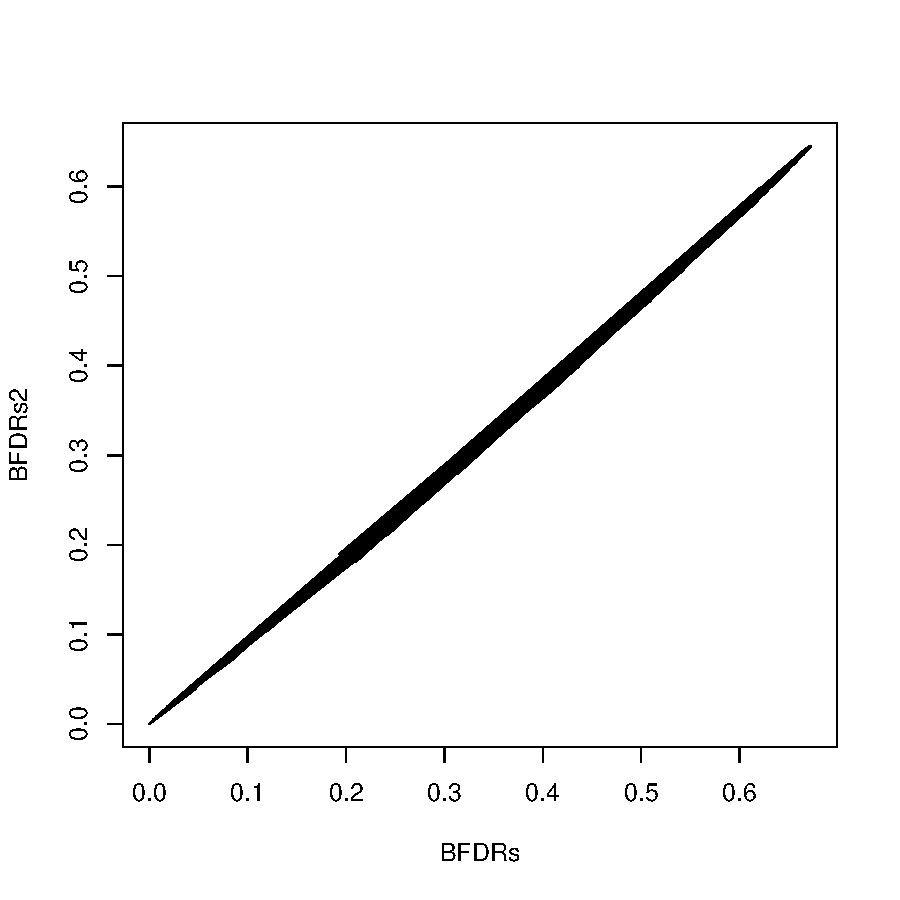
\includegraphics{ShrinkBayes-030}


\noindent
We observe they are very similar in this setting, hence the inference results are robust against misspecification
of the prior in this setting.


\section{Example 2: Gaussian setting, HT RNAi data}\label{htrnai}
\begin{Schunk}
\begin{Sinput}
> library(ShrinkBayes)
> data(HTRNAi)
> head(HTRNAi)
\end{Sinput}
\begin{Soutput}
                s1         s2         s3          s4         s5         s6
siRNA1  0.54317601  0.1953989  0.3883244 -0.03428689  0.6049207 -0.1790861
siRNA2  0.63533948  0.5057837  0.3928841  0.25338641  0.6935488  0.4185978
siRNA3 -0.91691878 -1.0838714 -0.6184123 -1.31090945 -0.2335765 -1.0377135
siRNA4 -0.74854963 -0.7619164 -0.2532474 -1.06233410 -0.5529374 -0.8189226
siRNA5  0.01110011 -0.6777245  0.3444957 -0.78924657  0.3554455 -0.8163929
siRNA6  0.59106644  0.5445666  0.4172433  0.31420140  0.6532168  0.5535300
\end{Soutput}
\end{Schunk}
Loads the package and the data

\para
\begin{Schunk}
\begin{Sinput}
> ncpus2use <- 10
\end{Sinput}
\end{Schunk}
Sets the number of cpus to use for parallel computations.

\para
\begin{Schunk}
\begin{Sinput}
> treatment <- factor(rep(c("untreated","treated"),3))
> assay <- factor(rep(1:3,each=2))
\end{Sinput}
\end{Schunk}
Defines covariates ``treatment'' and ``assay'', corresponding to the columns of the HTRNAi data.

\para
\begin{Schunk}
\begin{Sinput}
> offsetvalue <- c(0.1703984, -0.6958495,  0.3079694, -0.5582785,
+ 0.2251210, -0.6411269)
\end{Sinput}
\end{Schunk}
Defines an offset (often not needed). In this particular example, the offsets are computed from
HT RNAi data with a positive control which is run for the same 6 screens. The offsets are posterior mean estimates from the same model
as below (from many technical repeats per screen), but without shrinkage (because only one feature, the positive control, is involved). Use of an offset
guarantees that the parameter estimates can be intepreted as deviation from the positive control.


\para
\begin{Schunk}
\begin{Sinput}
> form = y ~ offset(offsetvalue) + 1 + treatment + assay
\end{Sinput}
\end{Schunk}
Define the model formula. Specification should be according to the {\tt inla formula} argument.

\para
\begin{Schunk}
\begin{Sinput}
> shrinksimul <- ShrinkGauss(form=form, dat=HTRNAi,shrinkfixed="treatment",
+ shrinkaddfixed="assay", fixedmeanzero = FALSE, ncpus=ncpus2use)
\end{Sinput}
\end{Schunk}

This function simultaneously shrinks the fixed effect parameters `treatment' and `assay'.
Note that in this particular setting it is likely that many treatment parameters are negative (since this concerns an effect with
respect to a positive control; see \citep{WielHTRNAi}). Therefore, we set {\tt fixedmeanzero = FALSE}, so that we do not fix the mean
of the prior
to zero (which is the logical default in many microarray settings).
In addition, the Gaussian error standard deviation is shrunken by default ({\tt shrinksigma = TRUE}).
This function may take considerable computing time.

The argument {\tt shrinkfixed} contains the parameter of primary interest (``treatment''), while {\tt shrinkaddfixed}
contains an additional (nuisance) parameter (``assay''). Currently, maximally two fixed effect parameters can be shrunken
simultaneously using Gaussian priors.
{\tt ShrinkGauss} has many additional arguments.
We discuss a few crucial ones.
\begin{itemize}
\item {\tt ntag}: Consecutive number of features used for shrinking. Important for computing time.
Default is {\tt ntag = c(100, 200, 500, 1000)}. You may
consider using smaller values (e.g. {\tt ntag = c(50, 100)}) for trying out, but we recommend to use at least {\tt 500} for final
computations.
\item {\tt maxiter}: Maximum number of iteration per value of {\tt ntag}. Important for computing time.
Default is 10. Consider using a smaller value for trying out, e.g. {\tt maxiter = 3}, but use at least {\tt maxiter=10} for final
computations.
\item {\tt fixedmeanzero} ({\tt addfixedmeanzero}): Should the Gaussian mean of the {\tt shrinkfixed} ({\tt shrinkaddfixed}) prior
    be fixed to 0?
Set to {\tt FALSE} when this is undesirable/unrealistic.
\end{itemize}


\para
\begin{Schunk}
\begin{Sinput}
> shrinksimul$pmlist
\end{Sinput}
\begin{Soutput}
$mufixed
[1] -0.4220818

$precfixed
[1] 15.22325

$muaddfixed
[1] 0

$precaddfixed
[1] 88.85478

$shaperand
[1] 0.001

$raterand
[1] 0.001

$mixp
[1] 0.2 0.8

$shapeerr
[1] 14.80563

$rateerr
[1] 0.9963235
\end{Soutput}
\end{Schunk}
Shows the final parameter values. Note that the second parameter of Gaussian priors is a precision (1/variance)
and the second parameter of Gamma priors (here, used for the precision of the error variance) is a rate.


\begin{Schunk}
\begin{Sinput}
> round(shrinksimul$paraall[,1:6],3)
\end{Sinput}
\begin{Soutput}
        mufixed precfixed muaddfixed precaddfixed shaperand raterand
paraall   0.000     0.100          0        0.100     0.001    0.001
paranew  -0.399     5.064          0        6.797     0.001    0.001
paranew  -0.405     7.761          0       13.148     0.001    0.001
paranew  -0.408     9.568          0       19.455     0.001    0.001
paranew  -0.407    10.626          0       25.331     0.001    0.001
paranew  -0.406    11.233          0       31.306     0.001    0.001
paranew  -0.406    11.657          0       36.715     0.001    0.001
paranew  -0.404    11.705          0       42.435     0.001    0.001
paranew  -0.406    11.478          0       47.533     0.001    0.001
paranew  -0.402    11.127          0       52.698     0.001    0.001
paranew  -0.406    10.904          0       57.092     0.001    0.001
paranew  -0.431    12.320          0       62.505     0.001    0.001
paranew  -0.444    13.260          0       66.303     0.001    0.001
paranew  -0.447    14.138          0       70.433     0.001    0.001
paranew  -0.447    14.877          0       74.258     0.001    0.001
paranew  -0.423    14.761          0       78.835     0.001    0.001
paranew  -0.420    15.117          0       82.779     0.001    0.001
paranew  -0.422    15.223          0       88.855     0.001    0.001
\end{Soutput}
\end{Schunk}

\begin{Schunk}
\begin{Sinput}
> round(shrinksimul$paraall[,-(1:6)],3)
\end{Sinput}
\begin{Soutput}
        mixp1 mixp2 shapeerr rateerr
paraall   0.2   0.8    0.001   0.001  NA
paranew   0.2   0.8    3.258   0.312 100
paranew   0.2   0.8    7.238   0.787 100
paranew   0.2   0.8    9.331   0.960 100
paranew   0.2   0.8   10.760   1.006 100
paranew   0.2   0.8   11.647   1.007 100
paranew   0.2   0.8   12.578   1.011 100
paranew   0.2   0.8   13.350   1.012 100
paranew   0.2   0.8   13.944   1.005 100
paranew   0.2   0.8   14.487   1.004 100
paranew   0.2   0.8   15.039   1.005 100
paranew   0.2   0.8   14.440   0.982 200
paranew   0.2   0.8   13.957   0.974 200
paranew   0.2   0.8   13.713   0.975 200
paranew   0.2   0.8   13.309   0.970 200
paranew   0.2   0.8   13.961   0.992 500
paranew   0.2   0.8   14.388   0.994 500
paranew   0.2   0.8   14.806   0.996 960
\end{Soutput}
\end{Schunk}
Shows the consecutive estimates of the parameters. Note that parameters not involved in the shrinkage are not updated.
The last columns shows the number of features used to estimate the parameters of the priors.

\para
\begin{Schunk}
\begin{Sinput}
> fitg <- FitAllShrink(form,dat=HTRNAi,fams="gaussian",shrinksimul,
+ ncpus=ncpus2use)
\end{Sinput}
\end{Schunk}
Applies {\tt inla} to compute posteriors for all data rows using the priors stored in {\tt shrinksimul}. IMPORTANT:
the prior for the {\tt shrinkfixed} parameter as used in {\tt ShrinkGauss} (here: ``treatment'') is by default dispersed
by a factor 10 (hence a vaguer prior is used). This is done, because we experienced that it leads to better results when
updating this prior to a nonparametric one (using {\tt NonParaUpdatePrior}) or a mixture one (using {\tt MixtureUpdatePrior}).
If you do not want to disperse the prior of the {\tt shrinkfixed} parameter, use the argument {\tt dispersefixed=1}.
Similar function arguments are available to disperse the prior of the {\tt shrinkaddfixed} parameter or (when available) the random
effects parameter. Additional arguments you may want to consider are {\tt showupdate} (default: {\tt FALSE}): when set to
{\tt TRUE} progression updates are shown for each {\tt updateby} finished features. However, this may slow down
the computations somewhat.

NOTE: you may see a lot of warnings from the call to inla. These usually occur for difficult data rows; this may either lead to
missing results (which the subsequent function can cope with) or very wide posteriors. In both cases, it is unlikely that
this leads to false positives or false negatives.

The result of {\tt FitAllShrink} is a 2-component list.
The first component {\tt \$res} is a list of {\tt inla}-output objects of length {\tt nr = nrow(dat)}, the number of data rows.
When {\tt nr} is large, the result may be a large object. Hence, for memory-efficiency not all inla-output is included.
See the function arguments {\tt effoutput}, {\tt keepmargrand} and {\tt keepmarghyper} for other options. The second component
{\tt \$priors} contains the input prior parameters.


\begin{Schunk}
\begin{Sinput}
> fit1 <- fitg$res[[1]]
\end{Sinput}
\end{Schunk}
Retrieves the {\tt inla}-output for the first feature. This contains a lot of information, including
marginal posteriors of all relevant parameters in numeric format; summaries of the posteriors; model fit summaries; input arguments
used by
{\tt inla}. Below we illustrate a few useful outputs.

\begin{Schunk}
\begin{Sinput}
> fit1$summary.fixed
\end{Sinput}
\begin{Soutput}
                     mean    sd 0.025quant 0.5quant 0.975quant      kld
(Intercept)         0.758 0.192      0.378    0.758     1.1300 7.40e-32
treatmentuntreated -0.353 0.203     -0.752   -0.353     0.0463 0.00e+00
assay2             -0.247 0.223     -0.683   -0.248     0.1950 1.23e-32
assay3             -0.142 0.223     -0.578   -0.143     0.2990 0.00e+00
\end{Soutput}
\end{Schunk}
Shows the summaries of the fixed effect parameters.

\begin{Schunk}
\begin{Sinput}
> marginal <- fit1$marginals.fixed$treatmentuntreated
> plot(marginal)
\end{Sinput}
\end{Schunk}
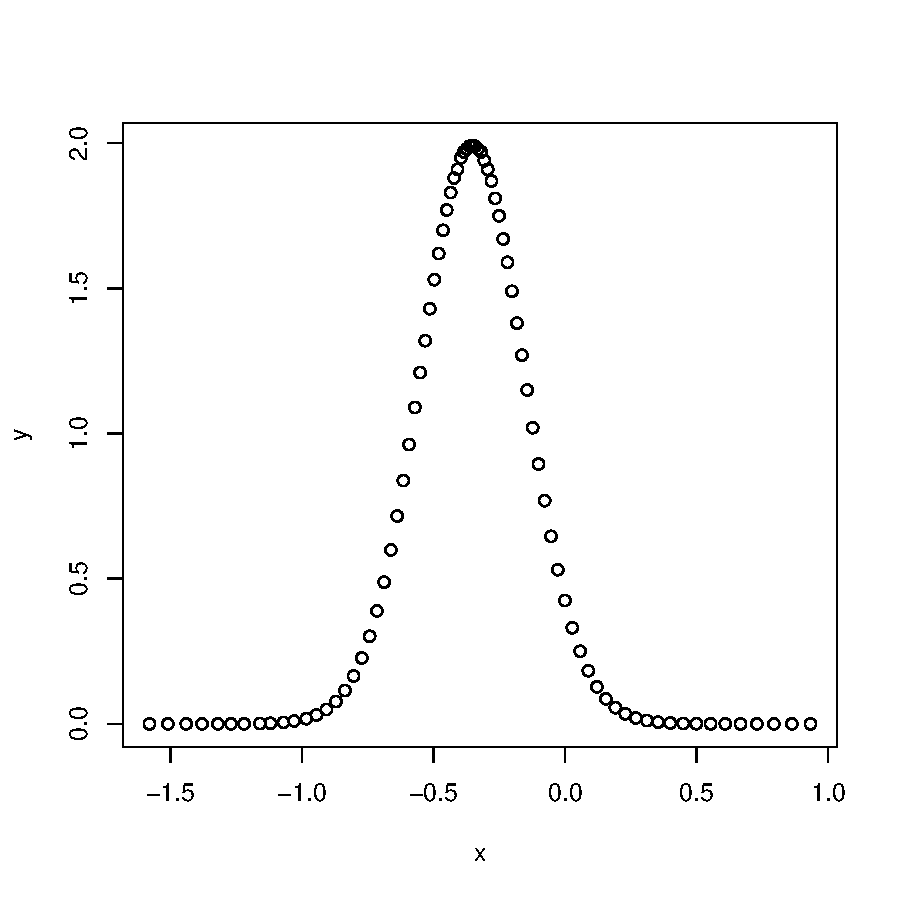
\includegraphics{ShrinkBayes-045}

\noindent
Plots the marginal posterior (Use {\tt type="l"} to obtain a curve instead of points). Note that this is obtained
under a prior the variance of which is dispersed with a factor 10.

\begin{Schunk}
\begin{Sinput}
> fit1$summary.hyper
\end{Sinput}
\begin{Soutput}
                                        mean   sd 0.025quant 0.5quant 0.975quant
Precision for the Gaussian observations 15.6 3.88       9.12     15.2       24.3
\end{Soutput}
\end{Schunk}
Shows the summaries of the hyper-parameters (parameters not involved in the regression formula).
In this case only the error variance is a hyper-parameter.

\begin{Schunk}
\begin{Sinput}
> fit1$mlik
\end{Sinput}
\begin{Soutput}
                                      [,1]
log marginal-likelihood (integration) -6.7
log marginal-likelihood (Gaussian)    -6.7
\end{Soutput}
\end{Schunk}
Estimation of the marginal likelihood. Can be used to compare models.

\begin{Schunk}
\begin{Sinput}
> npprior <- NonParaUpdatePrior(fitall=fitg,modus="fixed",
+ shrinkpara="treatment",ncpus=ncpus2use, includeP0=FALSE,
+ allow2modes=FALSE, symmetric=FALSE, logconcave=TRUE)
\end{Sinput}
\end{Schunk}
Updates the (dispersed) Gaussian prior for {\tt "treatment"} to a smooth, log-concave non-parametric one. Note here we specifically
allow an asymmetric prior (default is {\tt symmetric=TRUE}). Also, in this example, we do not include a point mass on zero, because the
main mass of effect sizes may well be concentrated elsewhere.
This is context specific. See \cite{WielHTRNAi} for explanation.
Dropping the symmetry requirement may cause the non-parametric prior to become more unstable (its tails may become too dependent on
specific data). Adding {\tt logconcave=TRUE}, which forces a log-concave prior \citep{Dumbgen2011}, aids in increasing the stability.


\para
Let us now compare the resulting non-parametric prior with the original Gaussian one.

\begin{Schunk}
\begin{Sinput}
> plot(npprior$priornew,type="l")
> supp <- npprior$priornew[,1]
> points(supp,dnorm(supp,mean=shrinksimul$pmlist$mufixed,
+ sd  = 1/sqrt(shrinksimul$pmlist$precfixed)),type="l",col="red",lty=2)
\end{Sinput}
\end{Schunk}
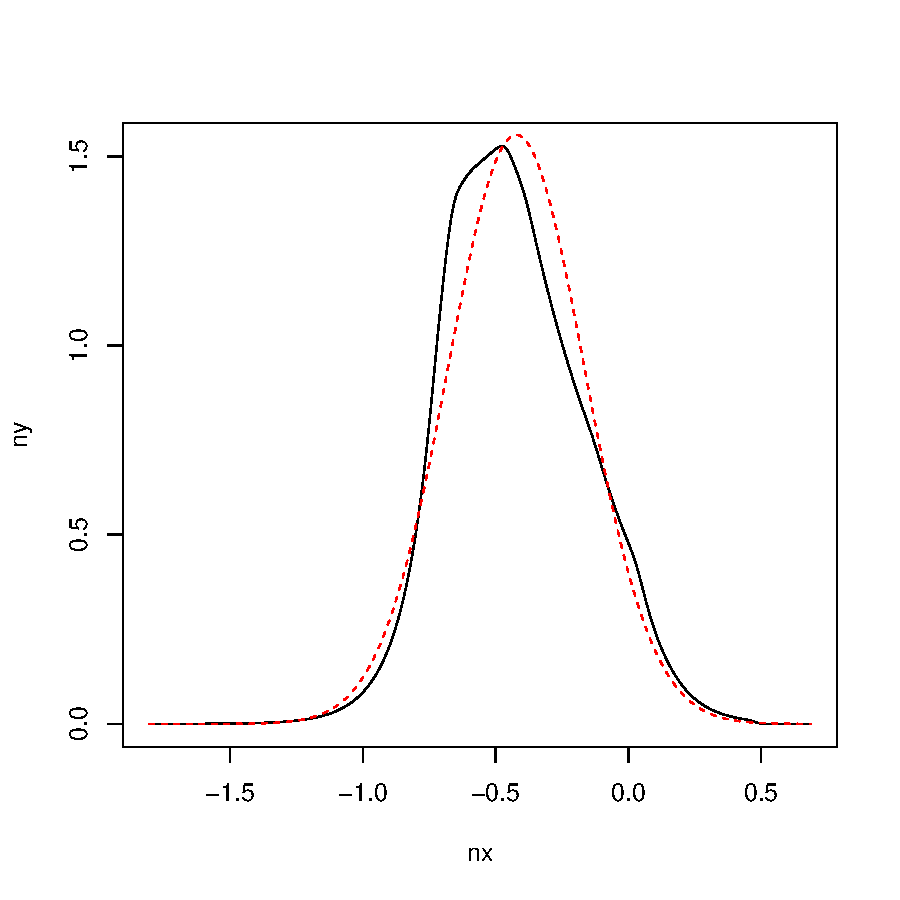
\includegraphics{ShrinkBayes-049}
\noindent
We observe a clear asymmetry and a difference in the tails.


\begin{Schunk}
\begin{Sinput}
> nppostshr <- NonParaUpdatePosterior(fitg,npprior,ncpus=ncpus2use)
\end{Sinput}
\end{Schunk}
Updates the posteriors of the {\tt "treatment"} parameter using the new, non-parametric prior.

\begin{Schunk}
\begin{Sinput}
> lfdr <- SummaryWrap(nppostshr, thr = 0, direction="lesser")
\end{Sinput}
\end{Schunk}
Here, we compute one-sided posterior null-probabilities of the kind {\tt lfdr} = $P(\beta_{\text{treat}} \leq 0 | Y)$, which can be
interpreted as a local false discovery rate.  One-sided, because, when comparing with a positive control, we are mainly interested
in siRNAs with larger (hence positive) effects w.r.t. the positive control, so {\tt lfdr} should be small.

\begin{Schunk}
\begin{Sinput}
> BFDRs <- BFDR(lfdr)
\end{Sinput}
\end{Schunk}
Computes Bayesian False Discovery Rates \citep{Ventrucci} from
the lfdrs.

\begin{Schunk}
\begin{Sinput}
> whsig <- which(BFDRs <= 0.1)
> whsig
\end{Sinput}
\begin{Soutput}
[1] 176 608 749
\end{Soutput}
\begin{Sinput}
> BFDRs[whsig]
\end{Sinput}
\begin{Soutput}
[1] 0.07658634 0.01426447 0.03969088
\end{Soutput}
\begin{Sinput}
> layout(matrix(1:3,nrow=1))
> plot(nppostshr[[whsig[1]]][[1]][[1]],xlim=c(-0.5,0.7),type="l")
> abline(v=0,lty=2)
> plot(nppostshr[[whsig[2]]][[1]][[1]],xlim=c(-0.5,0.7),type="l")
> abline(v=0,lty=2)
> plot(nppostshr[[whsig[3]]][[1]][[1]],xlim=c(-0.5,0.7),type="l")
> abline(v=0,lty=2)
\end{Sinput}
\end{Schunk}
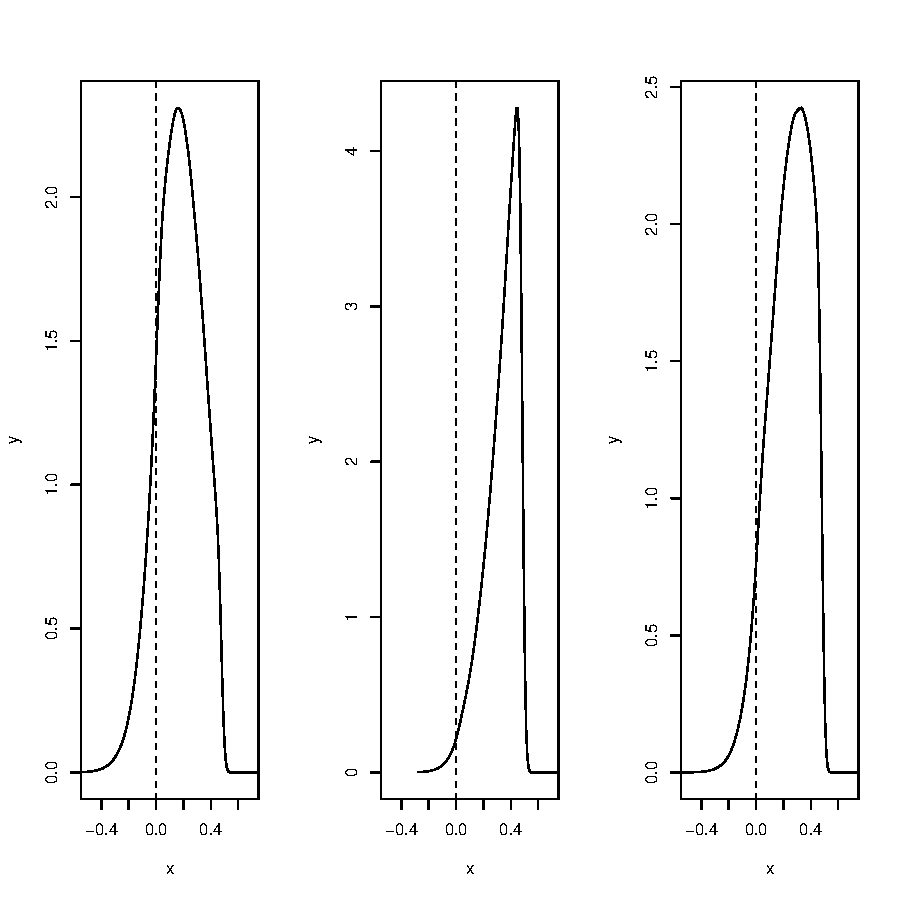
\includegraphics{ShrinkBayes-053}

\noindent Displays the posteriors of the significant siRNAs.
Note that use of a Gaussian prior rather than a non-parametric
one would have rendered only the second siRNA (id: 608) to be
significant (see \cite[]{WielHTRNAi}).


\section{Example 3: CAGE data}\label{cage}
The CAGE data set below consists of normalized sequencing (count) data for 10,000 tag clusters and 25 brain samples.
For illustration purposes we limit ourselves to the analysis of the first 1,000 tag clusters. Details on the analysis
are available in \cite{WielShrinkSeq} which present the results on 10,000 tag clusters.

\begin{Schunk}
\begin{Sinput}
> library(ShrinkBayes)
> data(CAGEdata10000)
> CAGEdata <- CAGEdata10000
> CAGEdata <- CAGEdata[1:1000,]
> CAGEdata[1:2,]
\end{Sinput}
\begin{Soutput}
      raw.0325_Frontal raw.0325_Hippocampus raw.0325_Putamen raw.0325_Temporal raw.034_Caudate raw.034_Frontal raw.034_Hippocampus
Tag.1                0                    0                0                 0              17               0                   0
Tag.2                0                    0                0                 0               4               0                   0
      raw.034_Temporal raw.05217_Caudate raw.05217_Frontal raw.05217_Hippocampus raw.05217_Putamen raw.05217_Temporal
Tag.1                0                76                68                    73                49                 57
Tag.2                0                10                 7                     4                 8                  6
      raw.05269_Caudate raw.05269_Frontal raw.05269_Hippocampus raw.05269_Putamen raw.05269_Temporal raw.07319_Frontal
Tag.1                 0                 0                    35                 0                  0                 0
Tag.2                 0                 0                     8                 0                  0                 0
      raw.07319_hippocampus raw.07319_Temporal raw.96373_Caudate raw.96373_Putamen raw.97266_Caudate raw.97266_Putamen
Tag.1                     0                  0                31                49                31                55
Tag.2                     0                  0                12                12                 7                 6
\end{Soutput}
\end{Schunk}
Load {\tt ShrinkBayes}, the data, select the first 1,000 rows and display the first 2.

\begin{Schunk}
\begin{Sinput}
> data(design_brain)
> design_brain
\end{Sinput}
\begin{Soutput}
   pers batch groupfac
1     1     0        2
2     1     0        3
3     1     0        4
4     1     0        5
5     2     1        1
6     2     0        2
7     2     0        3
8     2     0        5
9     3     1        1
10    3     1        2
11    3     1        3
12    3     1        4
13    3     1        5
14    4     0        1
15    4     0        2
16    4     1        3
17    4     0        4
18    4     0        5
19    5     0        2
20    5     0        3
21    5     0        5
22    6     1        1
23    6     1        4
24    7     1        1
25    7     1        4
\end{Soutput}
\end{Schunk}
Loads the design of the brain study.

\begin{Schunk}
\begin{Sinput}
> pers <- design_brain$pers  #persons
> batch <-design_brain$batch   #batch
> groupfac <- design_brain$groupfac #group (= brain region)
\end{Sinput}
\end{Schunk}
Retrieves covariates from the design matrix.

\begin{Schunk}
\begin{Sinput}
> ncpus2use <- 10
\end{Sinput}
\end{Schunk}
Number of cpus to use in (parallel) computations. Note that this should be specified separately
for functions that allow parallel computations by the {\tt ncpus =} argument.

\begin{Schunk}
\begin{Sinput}
> groupfac <- BaselineDef("groupfac",baselinegroup="1")
\end{Sinput}
\end{Schunk}
The brain regions, coded by variable {\tt groupfac}, are our main parameters of interest.
As the design displays, we are in a multiple (>2) group setting. The function {\tt BaselineDef} allows the user to set
the baseline group, rather than let {\tt INLA} decide. Here, the second argument is the character equivalent of the current level
of the desired baseline group.

\para
By default only comparisons with the baseline are included in the computations of posteriors. Use the following convenience function to create the other
pair-wise comparisons for a given factor when this contains 3 or more levels (groups):
\begin{Schunk}
\begin{Sinput}
> lincombvec <- AllComp("groupfac")
\end{Sinput}
\end{Schunk}

\begin{Schunk}
\begin{Sinput}
> form = y ~ 1 + groupfac + batch + f(pers,model="iid")
\end{Sinput}
\end{Schunk}
Define the model formula. Specification should be according to the {\tt inla} formula argument.
Here {\tt batch} and {\tt group} are fixed effects, {\tt pers} is a random effect. Please consider
including offsets in formula (see Section \ref{offset}) when your data has different library sizes!


\begin{Schunk}
\begin{Sinput}
> shrinksimul <- ShrinkSeq(form=form, dat=CAGEdata,shrinkfixed="groupfac",
+ shrinkrandom="pers",mixtdisp=TRUE,ncpus=ncpus2use)
\end{Sinput}
\end{Schunk}
Simultaneous shrinkage for {\tt groupfac} and {\tt pers}. In addition, the negative binomial overdispersion is shrunken
by default (see {\tt shrinkdisp} argument). Here, {\tt batch} is not shrunken, because the effect of {\tt batch} may not be uniform accross
the range of counts.
In the example we allow a mixture prior for overdispersion ({\tt mixtdisp=TRUE}). This increases the computing time by a factor 2,
because {\tt inla} has to fit the model under zero overdispersion (leading to a (zero-inflated) Poisson instead of a
zero-inflated negative binomial.) {\tt ShrinkSeq} default uses the zero-inflated negative binomial to fit sequencing data (see
\cite[]{WielShrinkSeq} for argumentation) by setting {\tt fams="zinb"}. However, other options are {\tt fams="nb", fams="poisson", fams="zip"} for
Negative Binomial, Poisson and zero-inflated Poisson, respectively. In case one opts for {\tt fams="nb"} it may be wise to
explicitly account for the relationship between the mean and the overdispersion when shrinking (see e.g. \cite[]{Huber2010}).
In {\tt ShrinkSeq} this is effectuated by setting {\tt curvedisp=TRUE}.
See the discussion on the {\tt ShrinkGauss} function in Section \ref{htrnai} for other important arguments of the function.



\begin{Schunk}
\begin{Sinput}
> shrinksimul$pmlist$mixp
\end{Sinput}
\begin{Soutput}
[1] 0.08376754 0.91623246
\end{Soutput}
\end{Schunk}
This returns the prior mass on the point mass of the mixture prior for overdispersion. If this would be close
to zero (which we have observed in some other RNAseq applications), then it is sufficient to fit the model on all data
for the (zero-inflated) Negative Binomial only. Otherwise, fits under the (zero-inflated) Poisson are also needed, like for this data set.


\begin{Schunk}
\begin{Sinput}
> fitzip <- FitAllShrink(form,dat=CAGEdata,fams="zip",shrinksimul,
+ ncpus=ncpus2use,lincomb=lincombvec)
\end{Sinput}
\end{Schunk}
Fits the model on all data using the priors resulting from ShrinkSeq and Zero-Inflated-Poisson likelihood. Note that, as discussed in Section
\ref{htrnai}, by default the variance of the prior for the main parameter of interest (here {\tt "groupfac"}) is increased by a factor 10.
The {\tt lincomb=lincombvec} argument specifies that the function should also generate posteriors for the linear combinations defined above.

\begin{Schunk}
\begin{Sinput}
> fitzinb <- FitAllShrink(form,dat=CAGEdata,fams="zinb",shrinksimul,
+ ncpus=ncpus2use,lincomb=lincombvec)
\end{Sinput}
\end{Schunk}
As above, but now under the Zero-Inflated-Negative Binomial likelihood (using the shrunken Gaussian prior for log-overdispersion).


\begin{Schunk}
\begin{Sinput}
> cp <- CombinePosteriors(fitzip,fitzinb,shrinksimul,para="groupfac",
+ ncpus=ncpus2use)
\end{Sinput}
\end{Schunk}
Combines the posteriors of the two fits (as outlined in the Suppl. Mat. of \cite[]{WielShrinkSeq}) for the {\tt "groupfac"} parameters and
the linear combinations  (included by default). Hence, {\tt cp} contains the posteriors of all pairwise comparisons under 1) a shrunken mixture prior
for overdispersion; 2) a shrunken Gamma prior for the precision of {\tt pers}; and 3) a (deliberately too wide) Gaussian prior
for {\tt "groupfac"}. The latter will now be updated to a non-parametric prior.

\begin{Schunk}
\begin{Sinput}
> npprior <- NonParaUpdatePrior(fitall=cp,modus="fixed", shrinkpara="groupfac",
+ shrinklc=names(lincombvec),lincombs=lincombvec,ncpus=ncpus2use, maxiter=3,
+ includeP0 = FALSE, symmetric = TRUE, allow2modes=FALSE)
\end{Sinput}
\end{Schunk}
Find one common nonparametric prior for all group-wise differences, including the contrasts defined in {\tt lincombvec}. Note that
if {\tt shrinklc} contains multiple contrasts, it is assumed they have the same mean and variance.
If you do not want to include those contrasts (e.g. because you are focusing on comparison with the baseline group), set
{\tt shrinklc=NULL} (default). Note that we advise to increase {\tt maxiter} for obtaining final results (default = 15).
Important other arguments and defaults of the {\tt NonParaUpdatePrior} function:
\begin{itemize}
\item {\tt includeP0 = TRUE}: Include a point mass?
\item {\tt symmetric = TRUE}: Force the prior to be symmetric?
\item {\tt unimodal = TRUE}: Force the prior to be unimodal?
\item {\tt allow2modes = FALSE}: Can the prior have one mode on both the postive and negative halfplane (so unimodal on both half planes)?
Only relevant when {\tt unimodal = TRUE}.
\item {\tt logconcave = FALSE}: Force the prior to be logconcave?
\end{itemize}
Note that here we use the default setting for the shape of prior (symmetric, unimodal, but not necessarily logconcave).
See also Section \ref{practical} for guidelines on how to use these settings.

\para
Let's have a look at the prior.
\begin{Schunk}
\begin{Sinput}
> theprior <- npprior$priornew
> plot(theprior,type="l",xlim=c(-2.5,2.5))
\end{Sinput}
\end{Schunk}
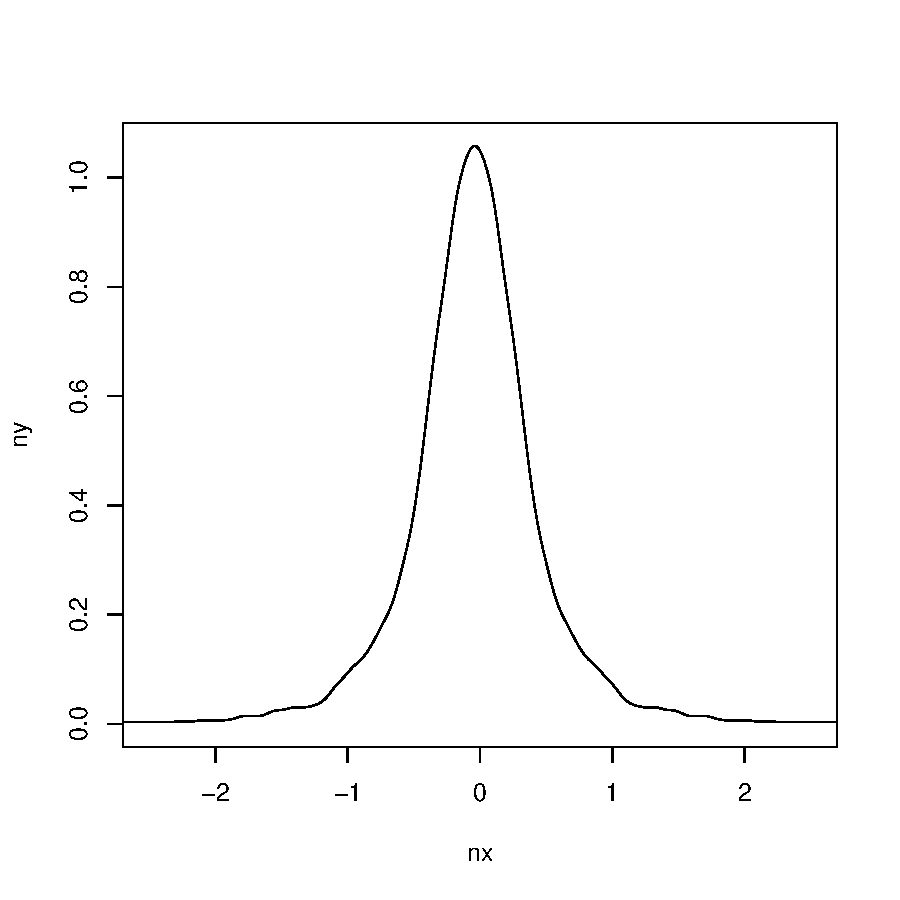
\includegraphics{ShrinkBayes-069}

\begin{Schunk}
\begin{Sinput}
> quantiles <- inla.qmarginal(p=c(0.05,0.25,0.5,0.75,0.95), theprior)
> quantiles
\end{Sinput}
\begin{Soutput}
[1] -0.92262861 -0.30907530 -0.04458935  0.21989661  0.83344991
\end{Soutput}
\begin{Sinput}
> expect <- inla.emarginal(function(x) x, theprior)
> expect
\end{Sinput}
\begin{Soutput}
[1] -0.03955675
\end{Soutput}
\begin{Sinput}
> sd <- sqrt(inla.emarginal(function(x) x^2, theprior) - expect^2)
> sd
\end{Sinput}
\begin{Soutput}
[1] 0.7232569
\end{Soutput}
\end{Schunk}
Computes quantiles, the mean and standard deviation of the prior. These functions can also be applied
to posteriors. See \texttt{?inla.qmarginal} and \texttt{?inla.emarginal} in your R-console for other options.

\begin{Schunk}
\begin{Sinput}
> nppostshr <- NonParaUpdatePosterior(cp,npprior,ncpus=ncpus2use)
\end{Sinput}
\end{Schunk}
Updates the posteriors of the {\tt "groupfac"} parameters and the contrasts involved in {\tt lincombvec}
using the new, non-parametric prior.


\begin{Schunk}
\begin{Sinput}
> lfdr <- SummaryWrap(nppostshr, thr = log(1.5))
\end{Sinput}
\end{Schunk}
Compute {\it two-sided} local fdrs
which equals lfdr = $\min(P(\beta_{\text{contrast}} \leq \text{thr}|Y), P(\beta_{\text{contrast}} \geq -\text{thr}|Y))$.
The above lfdr introduces a desirable conservativeness with respect to
an alternative posterior null-probability: lfdr' = $P(-\text{thr} \leq \beta_{\text{contrast}} \leq \text{thr}|Y)$. The latter, lfdr',
can not properly deal with wide posteriors that have a lot of probability mass outside $(-\text{thr},\text{thr})$.
See \cite{WielShrinkSeq} for further discussion. The threshold {\tt thr = log(1.5)} implies that we only wish to detect effects larger
than 1.5 fold (see Section \ref{practical}).


\begin{Schunk}
\begin{Sinput}
> BFDRs <- BFDR(lfdr)
\end{Sinput}
\end{Schunk}
\begin{Schunk}
\begin{Sinput}
> head(BFDRs)
\end{Sinput}
\begin{Soutput}
     groupfac2 groupfac3 groupfac4 groupfac5 groupfac3mingroupfac2 groupfac4mingroupfac2 groupfac4mingroupfac3
[1,] 0.7594013 0.7955304 0.8160210 0.8068468             0.8221437             0.8219757             0.8028797
[2,] 0.8278324 0.8494276 0.8345920 0.8368664             0.8288337             0.7963121             0.6930053
[3,] 0.8425993 0.1897167 0.7670844 0.8221101             0.1704118             0.5758759             0.8536606
[4,] 0.4884483 0.7963692 0.6165695 0.7589679             0.8493518             0.8409730             0.7933942
[5,] 0.8526093 0.8588785 0.8460374 0.8623392             0.8268282             0.7577407             0.6675664
[6,] 0.8008360 0.7607720 0.6496556 0.7627002             0.7307867             0.6133084             0.6748121
     groupfac5mingroupfac2 groupfac5mingroupfac3 groupfac5mingroupfac4
[1,]             0.8285386             0.8275530             0.8296039
[2,]             0.8182273             0.7975236             0.8355238
[3,]             0.7021078             0.8588213             0.8292926
[4,]             0.8438888             0.8152289             0.8396536
[5,]             0.8408789             0.8300127             0.8504250
[6,]             0.7305368             0.7452639             0.7984073
\end{Soutput}
\end{Schunk}
Compute (two-sided) Bayesian FDRs for all comparisons. Hence, a matrix is returned which features as rows and
comparisons as columns.

\begin{Schunk}
\begin{Sinput}
> BFDRmult <- BFDR(lfdr,multcomp=TRUE)
\end{Sinput}
\end{Schunk}

Compute (two-sided) Bayesian FDRs for testing the hypothesis: all comparisons parameters belong to the null domain.
This allows one to perform $K$-group inference (like in ANOVA or an F-test) using a multiple comparison set-up. Hence,
{\tt BFDRmult} may be used to discover features showing at least one difference between groups (but not where: for that {\tt BFDRs}
is needed.)

\begin{Schunk}
\begin{Sinput}
> wh <- which(BFDRmult <= 0.1)
> length(wh)
\end{Sinput}
\begin{Soutput}
[1] 43
\end{Soutput}
\end{Schunk}

\begin{Schunk}
\begin{Sinput}
> whcomp <- which(BFDRs[wh,]<= 0.1,arr.ind=TRUE)
> plot(cbind(whcomp[,2],wh[whcomp[,1]]),type="p",xlab="Comparison",
+ ylab="Feature index",xaxt="n")
> axis(1,at=1:10,labels=c("1-2","1-3","1-4","1-5","2-3","2-4","3-4",
+ "2-5","3-5","4-5"))
\end{Sinput}
\end{Schunk}
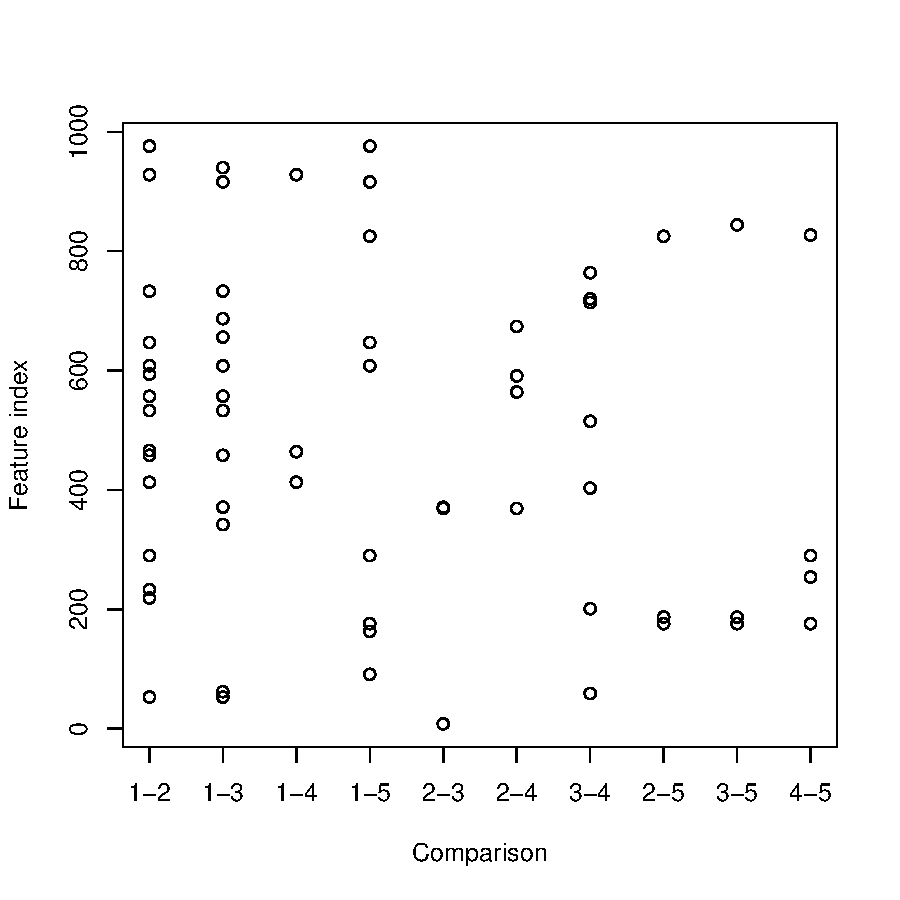
\includegraphics{ShrinkBayes-077}

\noindent
A plot that visualizes which features are significant for at least one comparison (hence according to
{\tt BFDRmult}) and which comparison is significant for those features (according to {\tt BFDRs}).

\section{Practical considerations to guide choices in the analysis workflow}\label{practical}
\subsection{Trying {\tt ShrinkBayes} on your data}
Analysing data should not contain too many `trial-and-error' steps, so ideally
data analysis settings should be fixed a priori. Nevertheless, in particular in complex data analysis problems,
it is often unavoidable that the researcher needs to try a few settings to understand what are sensible choices
for the data at hand. We advise to use a limited number of {\it randomly} selected features to try the various
functions and setting in {\tt ShrinkBayes}. The random selection is important, because many data sets contain structures
on the features (e.g. genomic ordering). In our experience, 1,000 features is a safe choice for the algorithms to work well, for
the results to be representative of the entire data set and computing times to be reasonable (in particular when processing on a multi-core
computer).

\para
We realize that the flexibility created by the many options in some of the functions in {\tt ShrinkBayes} comes at a price:
the (unexperienced) user may find it hard to make informed choices. Naturally, we assist the user on this issue by setting sensible
defaults. Here, we share practical tips that should further aid in practical use of {\tt ShrinkBayes}.

\subsection{To shrink or not to shrink?}
Shrinkage of a parameter can be beneficial in three ways.
In small sample settings dispersion parameters are generally difficult to estimate. Hence, there is reasonable consensus
on the benefit of shrinking dispersion-related parameters. This is effectuated in the functions {\tt ShrinkSeq} and {\tt ShrinkGauss} by the defaults
{\tt shrinkdisp = TRUE} and {\tt shrinksigma = TRUE}, respectively. For the main parameter of interest we argued that
shrinkage is important to come to proper inference in a Bayesian multiple testing setting \citep{WielShrinkSeq}. Hence, we strongly advise
to shrink this parameter or these parameters as well.

\para
For additional nuisance parameters in the regression the potential beneficial effect is
more subtle. In \cite{WielHTRNAi} we showed that shrinkage of the nuisance parameter {\tt "assay"} was very beneficial for more powerful inference for the
parameter of interest {\tt "treatment"}. The rationale for this was that in this experiment {\tt "assay"}, which had three levels, consumed 2 `degrees-of-freedom' (dof)\footnote{between quotes,
because, strictly, dof is not a Bayesian concept}, which is a lot in a 2*3 experiment. We found that the fitted prior for {\tt "assay"} was
very concentrated around zero, which basically renders more dof for the {\tt "treatment"} parameter. Hence, in very small experiments with a nuisance parameter
that has relatively many levels, it may certainly pay off to shrink the nuisance parameter. However, sometimes
the effect of the nuisance parameter is not uniform across the range of data, even after normalization. This may be assessed by plotting a (naive) estimate of the nuisance parameter
against the mean of the data (mean(log(x+1)) for when x is a count). In the HTRNAi example, Section \ref{htrnai}, the batch effect was not uniform
and so we decided not to shrink this. Since the zero-inflation parameter is also not uniform over the log-count range, we recommend to not shrink it
either (hence {\tt shrinkp0 = FALSE} is the default in {\tt ShrinkSeq}; see also \cite{WielShrinkSeq}).


\subsection{Paired data}
Paired data may be modeled in various ways. Currently, we recommend to model directly the data (so not the pairwise differences) and
account for the pairing by use of a random effect, similar to the use of {\tt pers} in the CAGE example of Section \ref{cage}. So for
5 individuals with a paired measurement this would be coded as: {\tt indiv = c(1,1,2,2,3,3,4,4,5,5)} and {\tt f(indiv,model="iid")}, assuming the
columns of the data are ordered with respect to individuals.

\para When the pairs represent individuals, we suggest
replacing the (zero-inflated) Negative Binomial by a
(zero-inflated) Poisson for count data, by setting {\tt
fams="zip"} (or {\tt fams="poisson"}) in the functions {\tt
ShrinkSeq} and {\tt FitAllShrink}. The reason for this is that
the between individual variation (which is the motivation for
overdispersing the Poisson) is now accounted for by the
Gaussian random effect in the regression.

\subsection{Choice of the prior}
{\tt ShrinkBayes} has many options for the prior, in particular when it concerns the main parameter of interest.
In general, we recommend to use
\begin{itemize}
\item {\tt MixtureUpdatePrior} with {\tt modus = "mixt"} for testing the point null-hypothesis $H_0: \beta=0$. Extensive simulations have shown
that this leads to rather accurate (B)FDR estimation for a wide variety of true effect size distributions, while rendering good power properties.
Alternative: {\tt NonParaUpdatePrior} with {\tt  includeP0 = TRUE}, a non-parametric prior with point mass. Slightly worse (B)FDR estimation. Possibly somewhat
more power than  {\tt MixtureUpdatePrior} for very small sample size (e.g. $N=2*3$).
\item {\tt NonParaUpdatePrior} with {\tt  includeP0 = FALSE} when testing an interval null-hypothesis, e.g. using thresholds like {\tt thr = log(1.25), thr = log(1.5), thr = log(2)} (or the negatives hereof).
The non-parametric prior provides the best adaptivity
to the data. For example, in Section \ref{htrnai} we illustrate
the benefit of using a nonparametric prior over a Gaussian one
in a small-sample setting. Also we have shown in simulation
settings that a nonparametric prior can accurately recover
smooth parametric shapes \citep{WielShrinkSeq}.
\item {\tt ShrinkSeq} or {\tt ShrinkGauss} using the option {\tt excludefornull} in combination with {\tt BFUpdatePosterior} to test two nested models
that differ by more than one variable.

\end{itemize}



\para  We, and others \citep{Lewin2007},
noted that for some data sets, the point mass on zero in
mixture priors is estimated to be very low, irrespective of the shape of continuous components. In such cases we
advise to use the default lower bound 0.5 on the point mass component {\tt p0lower = 0.5 } in {\tt NonParaUpdatePrior}
to force some shrinkage towards 0, in combination
with using a threshold {\tt thr} different from zero in {\tt SummaryWrap} .




\subsection{When should I use {\tt mixtdisp=TRUE}?} The {\tt
ShrinkSeq} function allows one to use a mixture of Poisson and
Negative Binomial likelihood (or zero-inflated versions
thereof) by setting {\tt mixtdisp=TRUE}. When the experiment
involves sequencing data on independent individuals our
experience (and the consensus in the community) is that
overdispersion (to allow more variance between samples than the
Poisson does) is really needed, so for such studies we expect
that the majority of features prefers the Negative Binomial, so
in such a case we recommend to simply use the default {\tt
mixtdisp=FALSE}. However, if the experiment involves cell lines
(hence less variability is likely) or when the
between-individual variation is modeled by a random effect at
the regression level (see Section \ref{cage}) we advise to use
{\tt mixtdisp=TRUE}. If the estimate of the mixture proportion
({\tt shrinksimul\$pmlist\$mixp}, where {\tt shrinksimul} is the
object containing the output of {\tt ShrinkSeq}) is close to 0,
proceed with (zero-inflated) Negative Binomial. If it is close
to 1, proceed with (zero-inflated) Poisson. Otherwise, fit both
and use the {\tt CombinePosteriors} function (see Section
\ref{cage}).

\subsection{Shape of the nonparametric prior: logconcave, unimodal, symmetric}
In the function {\tt NonParaPriorUpdate} the options {\tt logconcave}, {\tt unimodal} and {\tt symmetric} allow one to
increase stability of the prior. Setting all these options to {\tt FALSE} renders the completely non-restrictive setting, where
all {\tt TRUE} gives the most restrictive setting. We recommend to use either of the following two settings:
a) The default: {\tt logconcave = FALSE}, {\tt unimodal = TRUE} and {\tt symmetric = TRUE}, where enforcing symmetry and unimodality
creates stability for the tails of the prior. b) {\tt logconcave = TRUE}, {\tt unimodal = TRUE} and {\tt symmetric = FALSE},
if asymmetry is considered realistic; the log-concavity restriction may then help to stabilize both tails of the prior.

\subsection{What threshold to use for testing (lfdr and BFDR
computation)?} In the function {\tt SummaryWrap} the threshold
argument {\tt thr} is important for determining the significant
features by lfdr or BFDR. To a large extent the discussion on
minimal relevant effect size (which is what {\tt thr}
represents, on log level) is a biological one. The more {\tt thr}
deviates from 0 the less features are detected, but those that
are detected are likely to be (relatively) relevant. We advise
to be careful with using {\tt thr = 0} in the two-sided,
non-parametric setting, because if the truth is sparse (or
near-sparse: many very small effects) it may render too many
false positives. In general, we believe it is wise to report
results for at least two values of {\tt thr}, e.g.{\tt
thr=log(1.25)} and {\tt thr=log(2)}, representing 1.25 and
2-fold changes.

\subsection{How to deal with extremely large data sets?}
For very large data sets, the internal memory of the computer may not suffice
to perform the fits for all features in one call. Hence, we advise to split
the three major tasks of {\tt ShrinkBayes}: a) Finding the correct priors;  b)
Computing the posteriors under those priors; and c) Inference (lfdr and BFDR computations).
a) is usually accurate enough when using
a random subset of features of size, say 10,000. For those computations, internal memory
is usually sufficient.
Then, for the computation of posteriors we advise to do this in batches and save intermediate results
on the hard-disk. Then, perform inference on summaries of those posteriors using {\tt SummaryWrap} and {\tt BFDR}.

\para
An example is included in the Appendix, Section \ref{large}.

\subsection{Tips for speeding up computations}
Several functions in {\tt ShrinkBayes} may take a while to run.
Therefore, we parallelized some of the most time-consuming computations, so
your computations will obviously be faster when increasing the number of avalable.
Note that computing time increases linearly with the number of features.

\para
Some more tips for speeding up computations:
\begin{itemize}
\item When starting to use {\tt ShrinkBayes} clean up the R-memory: either by re-starting R
or by using {\tt rm(list=ls());gc();}.
\item If you use Windows OS: consider switching to Linux. Due to the intensive interaction of {\tt inla} with the hard-disk,
we experienced that use of Linux instead of Windows (on the same computer) may speed up computations by a factor of 3-4.


\end{itemize}

%\section{About Bayes' Factors and the correspondence with lfdr}

\section{Future topics}
We plan to extent {\tt ShrinkBayes} in many directions.
\begin{itemize}
\item Other data types, in particular fractional data (on 0-1 scale), e.g. methylation
\item Longitudinal settings (multiple measurements over time)
\item Modelling and reporting joint posteriors rather than only marginal ones
\item $K$-sample inference (other than through multiple comparisons, which was illustrated in the Section \ref{cage})
\item ``Small'' multivariate GLM settings. Where ``small'' means: non-high-dimensional (at the level of the model)
\item ``Large'' multivariate penalized regression settings
\item Inference with point mass on zero and {\it nonparametric} continuous component
\item Using Bayes' Factors for inference in a multiplicity setting
\item ...
\end{itemize}
If you are interested in any of these topics, or when you feel these are essential for your application, please let us know.
We might have progressed and be able to share (preliminary) code with you.

\section{Appendix}\label{appendix}
\subsection{Code used for generating the simulated data set `datsim'}\label{simulation}

\begin{Schunk}
\begin{Sinput}
> #1500 rows (siRNAs), 8 samples, pi0 = 2/3
> datsim1 <- matrix(rnorm(8000,mean=0,sd=0.5),nrow=1000)
> meanvec <- matrix(rep(rnorm(500,0,1),4),nrow=500)
> datsim2 <- cbind(matrix(rnorm(2000,mean=0,sd=0.5),nrow=500),
+ matrix(rnorm(2000,mean=0,sd=0.5),nrow=500) + meanvec)
> datsim <- rbind(datsim1,datsim2)
\end{Sinput}
\end{Schunk}

\subsection{Code for simulated example}
\begin{Schunk}
\begin{Sinput}
> library(ShrinkBayes)
> data(datsim)
> ncpus2use <- 10
> group <- factor(c(rep("group1",4),c(rep("group2",4))))
> form = y ~  1 + group
> form0 = y ~ 1
> shrinksimul <- ShrinkGauss(form=form, dat=datsim,shrinkfixed="group",
+ ncpus=ncpus2use)
> fitg <- FitAllShrink(form,dat=datsim,fams="gaussian",shrinksimul,
+ ncpus=ncpus2use)
> fitg0 <- FitAllShrink(form0,dat=datsim,fams="gaussian",shrinksimul,
+ ncpus=ncpus2use)
> mixtprior2gauss <- MixtureUpdatePrior(fitall=fitg,fitall0=fitg0,
+ modus="mixt", shrinkpara="group",ncpus=ncpus2use)
> mixtpostshr <- MixtureUpdatePosterior(fitg,mixtprior2gauss,fitg0,
+ ncpus=ncpus2use)
> lfdrless <- SummaryWrap(mixtpostshr, thr = 0, direction="lesser")
> lfdrgreat <- SummaryWrap(mixtpostshr, thr = 0, direction="greater")
> BFDRs <- BFDR(lfdrless,lfdrgreat)
\end{Sinput}
\end{Schunk}

\subsection{Code for HTRNAi example}
\begin{Schunk}
\begin{Sinput}
> library(ShrinkBayes)
> data(HTRNAi)
> ncpus2use <- 10
> treatment <- factor(rep(c("untreated","treated"),3))
> assay <- factor(rep(1:3,each=2))
> offsetvalue <- c(0.1703984, -0.6958495,  0.3079694, -0.5582785,
+ 0.2251210, -0.6411269)
> form = y ~ offset(offsetvalue) + 1 + treatment + assay
> shrinksimul <- ShrinkGauss(form=form, dat=HTRNAi,shrinkfixed="treatment",
+ shrinkaddfixed="assay", fixedmeanzero = FALSE, ncpus=ncpus2use)
> fitg <- FitAllShrink(form,dat=HTRNAi,fams="gaussian",shrinksimul,
+ ncpus=ncpus2use)
> npprior <- NonParaUpdatePrior(fitall=fitg,modus="fixed",
+ shrinkpara="treatment", ncpus=ncpus2use, includeP0 = FALSE,
+ logconcave=TRUE, allow2modes=FALSE)
> nppostshr <- NonParaUpdatePosterior(fitg,npprior,ncpus=ncpus2use)
> lfdr <- SummaryWrap(nppostshr, thr = 0, direction="lesser")
> BFDRs <- BFDR(lfdr)
\end{Sinput}
\end{Schunk}

\subsection{Code for CAGE example}
\begin{Schunk}
\begin{Sinput}
> data(CAGEdata10000)
> CAGEdata <- CAGEdata10000[1:1000,]
> data(design_brain)
> pers <- design_brain$pers ; batch <-design_brain$batch;
> groupfac <- design_brain$groupfac
> ncpus2use <- 10
> groupfac <- BaselineDef("groupfac",baselinegroup="1")
> lincombvec <- AllComp("groupfac")
> form = y ~ 1 + groupfac + batch + f(pers,model="iid")
> shrinksimul <- ShrinkSeq(form=form, dat=CAGEdata,shrinkfixed="groupfac",
+ shrinkrandom="pers",mixtdisp=TRUE,ncpus=ncpus2use)
> fitzip <- FitAllShrink(form,dat=CAGEdata,fams="zip",shrinksimul,
+ ncpus=ncpus2use,lincomb=lincombvec)
> fitzinb <- FitAllShrink(form,dat=CAGEdata,fams="zinb",shrinksimul,
+ ncpus=ncpus2use,lincomb=lincombvec)
> cp <- CombinePosteriors(fitzip,fitzinb,shrinksimul,para="groupfac",
+ ncpus=ncpus2use)
> npprior <- NonParaUpdatePrior(fitall=cp,modus="fixed",
+ shrinkpara="groupfac", shrinklc=TRUE,ncpus=ncpus2use, maxiter=3,
+ includeP0 = FALSE, symmetric=TRUE, logconcave=FALSE, allow2modes=FALSE)
> nppostshr <- NonParaUpdatePosterior(cp,npprior,ncpus=ncpus2use)
> lfdr <- SummaryWrap(nppostshr, thr = log(1.5))
> BFDRs <- BFDR(lfdr)
> BFDRmult <- BFDR(lfdr,multcomp=TRUE)
\end{Sinput}
\end{Schunk}

\subsection{Code for running {\tt ShrinkBayes} on very large data sets: simulated example}\label{large}
\begin{Schunk}
\begin{Sinput}
> datsim1 <- matrix(rnorm(400000*8,mean=0,sd=0.5),nrow=400000)
> meanvec <- matrix(rep(rnorm(200000,0,1),4),nrow=200000)
> datsim2 <- cbind(matrix(rnorm(200000*4,mean=0,sd=0.5),nrow=200000),
+ matrix(rnorm(200000*4,mean=0,sd=0.5),nrow=200000) + meanvec)
> datsimlarge <- rbind(datsim1,datsim2)
> save(datsimlarge,file="datsimlarge.Rdata")
\end{Sinput}
\end{Schunk}
Simulates a data set with 600,000 rows, 4*2 samples, pi0 = 2/3. See Section \ref{simul}.


\begin{Schunk}
\begin{Sinput}
> tuningsize <- 10000
> batchsize <- 50000
\end{Sinput}
\end{Schunk}
{\tt tuningsize} determines the maximum
number of features used in the tuning phase of ShrinkBayes. The
tuning phase determines the priors for those parameters for
which shrinkage is desired. Then, the actual fitting and
computation of posteriors for all features is performed in
batches of size 'batchsize'. Results are written to the
hard-disk in batches. All this to avoid having to store many
posterior distributions in the internal memory.



\begin{Schunk}
\begin{Sinput}
> whrows <- sample(1:nrow(datsimlarge),tuningsize)
> datsimtune <- datsimlarge[whrows,]
> save(datsimtune,file="datsimtune.Rdata")
> rm(datsimlarge);gc()
\end{Sinput}
\end{Schunk}
Creates the tuning data set on a random set of features. {\tt datsimtune} is used to
fit the priors

\begin{Schunk}
\begin{Sinput}
> ncpus2use <- 6
> group <- factor(c(rep("group1",4),c(rep("group2",4))))
> form = y ~  1 + group
> form0 = y ~  1
> library(ShrinkBayes)
\end{Sinput}
\end{Schunk}
Number of cpus to use, covariate {\tt group}, formula and library loading

\begin{Schunk}
\begin{Sinput}
> shrinksimul <- ShrinkGauss(form=form, dat=datsimtune,shrinkfixed="group",
+ ncpus=ncpus2use)
> fitg <- FitAllShrink(form,dat=datsimtune,fams="gaussian",shrinksimul,
+ ncpus=ncpus2use)
> fitg0 <- FitAllShrink(form0,dat=datsimtune,fams="gaussian",shrinksimul,
+ ncpus=ncpus2use)
> mixtprior<- MixtureUpdatePrior(fitall=fitg, fitall0=fitg0,modus="gauss",
+ shrinkpara="group",ncpus=ncpus2use)
> save(shrinksimul,mixtprior,file="priorstuned.Rdata")
\end{Sinput}
\end{Schunk}
Determining the priors using the exact same code as in Section \ref{simul}, but now on the tuning data set {\tt datsimtune}.
Now, we start with fitting on the large data set.

\para
\begin{Schunk}
\begin{Sinput}
> saveFits <- FALSE
\end{Sinput}
\end{Schunk}
Do you want to save the inla-output of the function {\tt FitShrinkAll}? Note that these are large objects that contain
a lot of information, including marginal posteriors of all parameters.

\begin{Schunk}
\begin{Sinput}
> savePosteriors <- TRUE
\end{Sinput}
\end{Schunk}
Do you want to save output of the update function (either {\tt MixtureUpdatePosterior} or {\tt NonParaUpdatePosterior})?
This output contains the marginal posteriors of the parameter of interest only. May still be a fairly large object,
but generally much smaller than the fit object. Usually wise to store these in case you decide to change inference
in the {\tt SummaryWrap} and {\tt BFDR functions} (e.g. a different threshold).

\begin{Schunk}
\begin{Sinput}
> load("priorstuned.Rdata")
> load("datsimlarge.Rdata")
\end{Sinput}
\end{Schunk}
Load the R-objects that contain the information on the priors and the large data set.

\begin{Schunk}
\begin{Sinput}
> nr <- nrow(datsimlarge)
> nloop <- ceiling(nr/batchsize)
> lfdrless <- c()
> lfdrgreat <- c()
\end{Sinput}
\end{Schunk}
Determines the number of features, the number of loops and initializes the lfdrs

\begin{Schunk}
\begin{Sinput}
> for(k in 1:nloop){
+ if(k>1) load("datsimlarge.Rdata")
+ rangek <- ((k-1)*batchsize+1):min(nr,k*batchsize)
+ datk <- datsimlarge[rangek,]
+ print(paste("Computing posteriors for features",rangek[1],"to",
+ rangek[length(rangek)]))
+ rm(datsimlarge);gc()
+ fitgk <- FitAllShrink(form,dat=datk,fams="gaussian",shrinksimul,
+ ncpus=ncpus2use)
+ fitg0k <- FitAllShrink(form0,dat=datk,fams="gaussian",shrinksimul,
+ ncpus=ncpus2use)
+ if(saveFits) {
+     save(fitgk,file=paste("fitg_batch_",k,".Rdata",sep=""))
+     save(fitg0k,file=paste("fitg0_batch_",k,".Rdata",sep=""))
+     }
+ mixtpostshrk <- MixtureUpdatePosterior(fitgk,mixtprior,fitg0k,
+ ncpus=ncpus2use)
+ if(savePosteriors) save(mixtpostshrk,
+ file=paste("mixtpostshr_batch_",k,".Rdata",sep=""))
+ lfdrlessk <- SummaryWrap(mixtpostshrk, thr = 0, direction="lesser")
+ lfdrgreatk <- SummaryWrap(mixtpostshrk, thr = 0, direction="greater")
+ lfdrless <- rbind(lfdrless,lfdrlessk)
+ lfdrgreat <- rbind(lfdrgreat,lfdrgreatk)
+ save(lfdrless,lfdrgreat,file="lfdrs.Rdata")
+ rm(fitgk,mixtpostshr);gc()
+ }
\end{Sinput}
\end{Schunk}
The loop that determines posteriors for all features per batch of size {\tt batchsize}. {\tt FitAllShrink} determines the
posteriors under the initial priors stored in {\tt simulshrink}, {\tt MixtureUpdatePosterior} updates these posteriors
for the {\tt mixtprior} on {\tt "group"}.  Then lfdrs are computed for batch {\tt k} and all lfdrs are stored in
{\tt lfdrless} and {\tt lfdrgreat}.

\begin{Schunk}
\begin{Sinput}
> BFDRs <- BFDR(lfdrless,lfdrgreat)
\end{Sinput}
\end{Schunk}
Finally, BFDRs are computed. Note that these need the input of \emph{all} features, so BFDR cannot
be computed inside the loop above.

\subsection{Code used for True FDR in simulation setting}\label{truefdr}
{\tt negatives}: Indices of true negatives , {\tt sig}: BFDR measure of significance.
\begin{Schunk}
\begin{Sinput}
fdrcomp <- function(negatives,sig){
#True FDR = FP/N_P. Est FDR = \sum (p0s*I) / N_P
sortsig <- sort(sig,index.return=T)
sortind <- sortsig$ix
n <- length(sig)
arr <- rep(0,n)
wh <- which(sapply(sortind,is.element,set=negatives))
arr[wh] <- 1
FP <- cumsum(arr)
TrueFDR <- FP/1:n
EstFDR <- sortsig$x
return(cbind(TrueFDR,EstFDR))
}
\end{Sinput}
\end{Schunk}
\bibliographystyle{apalike}
\bibliography{C://Synchr//Bibfiles//bibarrays}
\end{document}
